\RequirePackage{fixltx2e}
\documentclass[a4paper,reprint,floatfix,amsmath,amssymb,aps,pra]{revtex4-1}

\usepackage{dragly-revtex}

\begin{document}

\title{FYS4460 Project 3}
\author{Svenn-Arne Dragly}

\begin{abstract}
In this project we are working with percolation, the study of connectivity and other properties in random media.
\end{abstract}

\maketitle

\section{Introduction}

Percolation is the study of connectivity and other properties in random media. We will in this project study a two-dimensional system where a binary matrix is chosen at random with a given probability $p$ for each of its sites to be occupied or not. These sites will be grouped into clusters which are studied for their connectivity, areas, masses and other properties. In this project, we will dig into topics such as percolation treshold and power law distributions.

\section{Theory}

\subsection{Definitions}

For the reference (and to give myself somewhere to look up stuff), I've listed the definitions used throughout this project in table \ref{tab:definitions}.
\begingroup
\begin{table}[ht]
\setlength\extrarowheight{4pt} % or whatever amount is appropriate
\begin{ruledtabular}
\begin{tabular}{l p{.31\textwidth}}
Term       &                  Definition \\
\hline
cluster & Set of sites that are connected \\
connected & Sites that share sides. In this project, we define connections with 4 neighbors on a square lattice \\
spanning cluster & A cluster that spans the whole system from edge to edge in either direction \\
finit cluster & Any cluster that is not a spanning cluster \\
\end{tabular}
\end{ruledtabular}
\caption{Definitions used throughout this project}
\label{tab:definitions}
\end{table}
\endgroup
\begin{table}
abc
\end{table}


There are also a set of properties that we will explore, such as the probability for a site to be part of the spanning cluster and the probability for a spanning cluster to exist at all. These are listed in table \ref{tab:properties}.
\begingroup
\begin{table}[ht]
\setlength\extrarowheight{4pt} % or whatever amount is appropriate
\begin{ruledtabular}
\begin{tabular}{l p{.37\textwidth}}
Property       &                  Definition \\
\hline
$p$             &       Probability that a site will be occupied. \\
$P(p, L)$       &       Probability that a site is part of the spanning cluster \\
$\Pi(p,L)$      &       Probability that a spanning cluster exists in the system \\
$g(r,p,L)$      &       Probability that two sites a distance $r$ apart belong to the same spanning cluster \\
$s$             &       Denotes the size of a cluster \\
$\xi(p,L)$      &       Correlation length \\
$sn(s,p,L)$     &       Probability for a site to belong to a cluster of size $s$. \\
$n(s,p,L)$      &       Cluster density - a useful property that among other things is used to find $sn(s,p,L)$ \\
$S(p)$          &       Average cluster size.

\end{tabular}
\end{ruledtabular}
\caption{Properties that will be explored in this project}
\label{tab:properties}
\end{table}
\endgroup

\subsection{One-dimensional percolation theory}

We use a few findings from one-dimensional percolation theory to build up our intuition for finite-dimensional percolation theory.

\subsubsection{Verifying the normalized density}
%
From one-dimensional percolation theory, we need to verify that $sn(s,p)$ is a normalized density. This is discussed in section 2.2 of the syllabus, and will be elaborated here for future reference.
\begin{equation}
  \sum_{s} sn(s,p) = \sum_{s=1}^{\infty} sp^{s} (1-p)^{2} = (1-p)^{2} p \sum_{s = 1}^{\infty} sp^{s-1}
\end{equation} 
Adding a term for $s = 0$ to the sum changes nothing because $0 \cdot p^{0 - 1} = 0$. This lets us rewrite the above as
\begin{equation}
  \sum_{s} sn(s,p) = (1-p)^{2} p \sum_{s = 0}^{\infty} sp^{s-1}.
\end{equation} 
This is written with the extra $p$ outside the sum to exploit the derivative of $p^s$,
\begin{equation}
  \sum_{s} sn(s,p) = (1-p)^{2} p \frac{d}{dp }\sum_{s = 0}^{\infty} p^{s}.
\end{equation}
Further, we use the summation rule $\sum_{s=0}^{\infty} p^s = 1/(1-p)$ to find
\begin{equation}
  \sum_{s} sn(s,p) = p.
\end{equation}
This shows that $sn(s,p)$ is a normalized density.

\section{Implementation}

Python has been used as the main programming language for this project. To do this, I needed to find the relevant functions to use in Python that corresponds to the listed functions in MATLAB.

\subsection{Working with percolation clusters in Python}
%
\emph{For the original article, see \href{http://dragly.org/2013/03/25/working-with-percolation-clusters-in-python/}{this webpage}.}

First of all, we need to include the pylab package together with the scipy.ndimage.measurements package:
%
\begin{lstlisting}
from pylab import *
from scipy.ndimage import measurements
\end{lstlisting}
%
Now, let's create a random matrix of filled and unfilled regions and visualize it:

\begin{lstlisting}
L = 100
r = rand(L,L)
p = 0.4
z = r<p

imshow(z, origin='lower')
colorbar()
title("Matrix")
show()
\end{lstlisting}
%
\begin{figure}
  \centering
  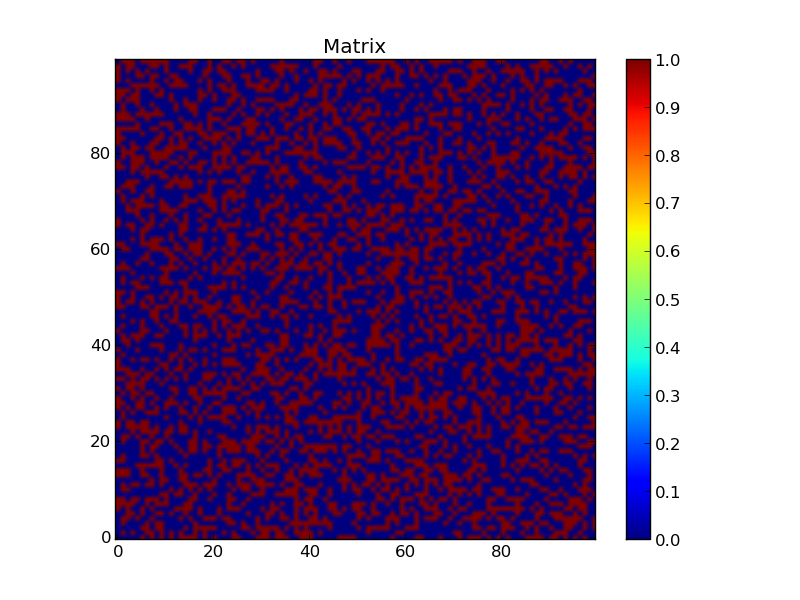
\includegraphics[width=0.35\textwidth]{./images/matrix.png}
  % matrix.png: 800x600 pixel, 100dpi, 20.32x15.24 cm, bb=0 0 576 432
  \caption{Example of a binary matrix that we'll perform our calculations on.}
  \label{fig:intro-matrix}
\end{figure}

This creates a matrix of random numbers r before creating a map z of this matrix where each element is set to True if $r < p$ and False if $r > p$ as shown in figure \ref{fig:intro-matrix}.

Furthermore we want to label each cluster. This is performed by the scipy.ndimage.measurements.label function:
%
\begin{lstlisting}
lw, num = measurements.label(z)
imshow(lw, origin='lower')
colorbar()
title("Labeled clusters")
show()
\end{lstlisting}
%
\begin{figure}[b]
  \centering
  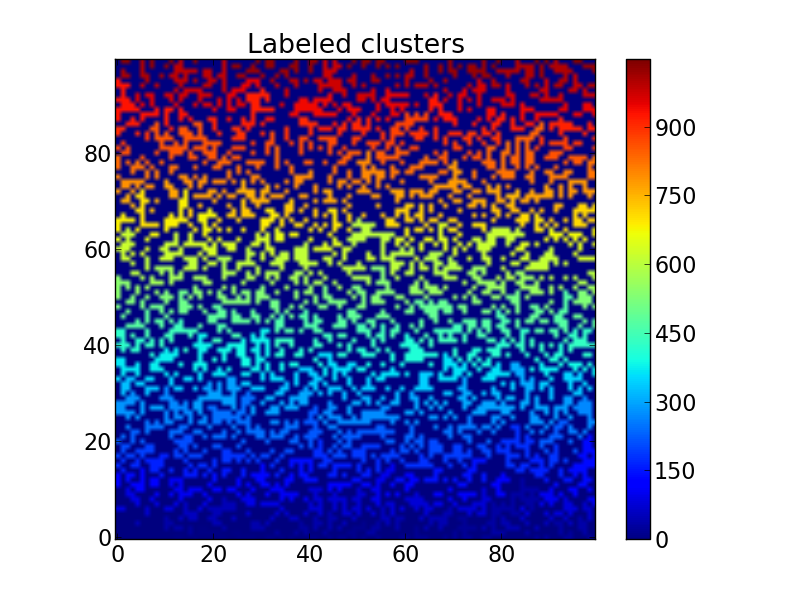
\includegraphics[width=0.35\textwidth]{./images/labeled-matrix-ordered.png}
  % matrix.png: 800x600 pixel, 100dpi, 20.32x15.24 cm, bb=0 0 576 432
  \caption{Matrix labels, with colors ordered from bottom to top.}
  \label{fig:intro-labels}
\end{figure}
%
This labels each cluster with a number which may be visualized using the imshow function as shown in figure \ref{fig:intro-labels}.

Beacause the label starts from the bottom up, the cluster colors are a bit too ordered, making it hard to distinguish two clusters close to each other. To fix this, we may shuffle the labeling with the following code:
%
\begin{lstlisting}
b = arange(lw.max() + 1)
shuffle(b)
shuffledLw = b[lw]
imshow(shuffledLw, origin='lower')
colorbar()
title("Labeled clusters")
show()
\end{lstlisting}
%
\begin{figure}
  \centering
  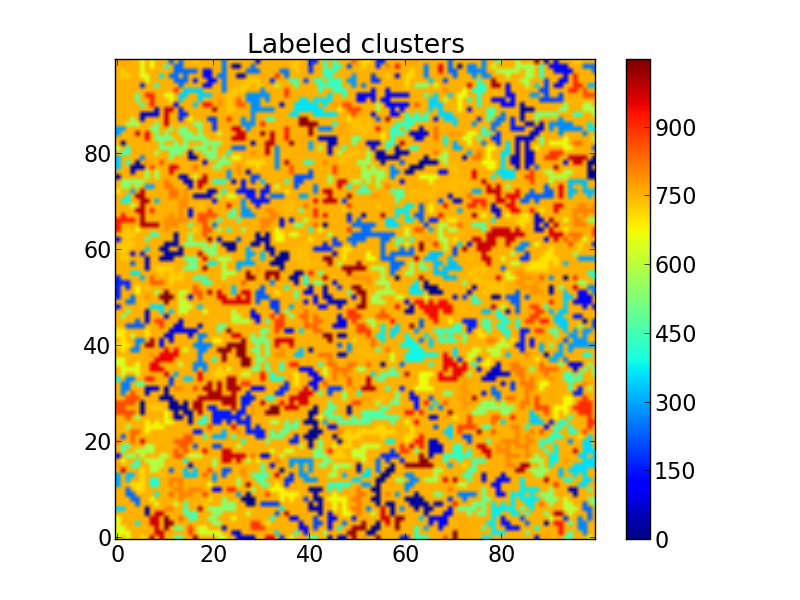
\includegraphics[width=0.35\textwidth]{./images/labeled-matrix.png}
  % matrix.png: 800x600 pixel, 100dpi, 20.32x15.24 cm, bb=0 0 576 432
  \caption{Matrix with labels in random order.}
  \label{fig:intro-better-labels}
\end{figure}
%
Now it is way easier to see the different clusters as shown in figure \ref{fig:intro-better-labels}.

After this we may want to extract some properties of the clusters, such as the area. This is possible using the scipy.ndimage.measurements.sum function:
%
\begin{lstlisting}
area = measurements.sum(z, lw, index=arange(lw.max() + 1))
areaImg = area[lw]
im3 = imshow(areaImg, origin='lower')
colorbar()
title("Clusters by area")
show()
\end{lstlisting}
%
The above code now plots the same matrix as above, but this time with all clusters colored by area.

Finally, we may want to find the bounding box of the largest cluster, so we again may see if there is a path from one side to the other. This is possible by using the function scipy.ndimage.measurements.find\_objects. Note however that this is a bit risky. If there are two clusters that are largest with the same area, find\_objects will find the bounding box of both clusters. That's why we'll need to rather loop over the labels for the clusters with max areas. This is done by the following code:
%
\begin{lstlisting}
labelList = arange(lw.max + 1)
maxLabels = labelList[where(area == area.max())]
for label in maxLabels:
  ...
\end{lstlisting}
%
In this for loop, we use the find\_objects function to plot a rectangle around the largest clusters:
%
\begin{lstlisting}
sliced = measurements.find_objects(lw == label)
if(len(sliced) > 0):
    sliceX = sliced[0][1]
    sliceY = sliced[0][0]
    plotxlim=im3.axes.get_xlim()
    plotylim=im3.axes.get_ylim()
    plot([sliceX.start, sliceX.start, sliceX.stop, sliceX.stop, sliceX.start], \
                      [sliceY.start, sliceY.stop, sliceY.stop, sliceY.start, sliceY.start], \
                      color="red")
    xlim(plotxlim)
    ylim(plotylim)

show()
\end{lstlisting}
%
\begin{figure}
  \centering
  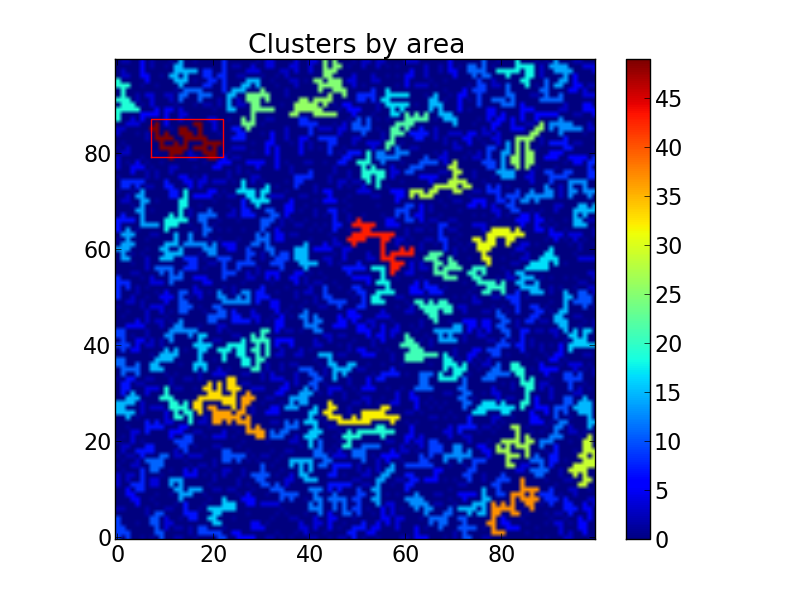
\includegraphics[width=0.35\textwidth]{./images/bounding-box.png}
  % matrix.png: 800x600 pixel, 100dpi, 20.32x15.24 cm, bb=0 0 576 432
  \caption{Matrix with clusters colored by area.}
  \label{fig:intro-final}
\end{figure}
%
This final plot is shown in figure \ref{fig:intro-final} and the whole script is located in \href{https://github.com/dragly/fys4460-project3}{the Git repository for this project}.

\subsection{Probability for a site to be part of the spanning cluster}

To find the probability for a site to be part of the spanning cluster, $P(p,L)$, I've iterated over different $p$ in the range $p=0.5$ to $p=1$ (by inspection, there was no reason to include values for $p<0.5$). For each $p$, the above program is run $1000$ times while the \textbf{sliceX} and \textbf{sliceY} variables are checked against the size of the whole matrix:
\begin{lstlisting}
if sliceX.stop - sliceX.start >= Lx or sliceY.stop - sliceY.start >= Ly:
    P = area.max() / (Lx * Ly)
else:
    P = 0
\end{lstlisting}
We then find the average of all $P$ for each $p$. In principle this could easily be extended to systems of rectangular shape. To extend it further to systems with for instance hexagonal boundaries or shearing, further steps would be needed to compare the edges of the boundaries to the spanning cluster. This is likely just a matter of some geometric operations, for instance creating bounding boxes near the boundaries and seeing if these intersect the edge or not. This has not been attempted in this project.

For the case with $L=100$, $P$ goes as a function of $p$ as shown in figure \ref{fig:P-vs-p}.
\begin{figure}
  \centering
  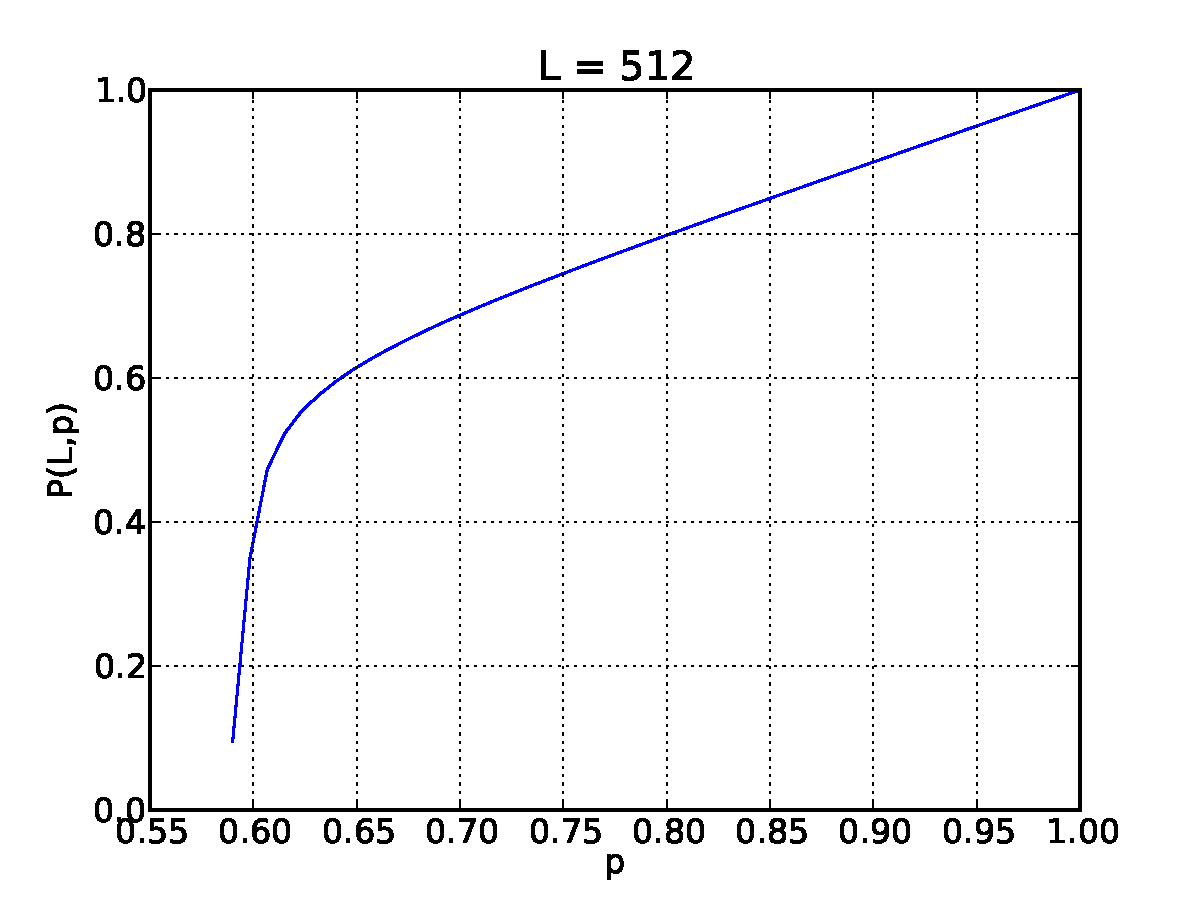
\includegraphics[width=0.45\textwidth]{../percolation/results/1a/P-vs-p-L512-nsamples500.pdf}
  % matrix.png: 800x600 pixel, 100dpi, 20.32x15.24 cm, bb=0 0 576 432
  \caption{Probability for a site to be part of the spanning cluster $P(p,L)$ plotted as a function of $p$. This was found by sampling $P$ for $500$ random binary matrices for different values of $p$.}
  \label{fig:P-vs-p}
\end{figure}

\subsection{The form of the function}

We now have an estimate for the probability for a site to be part of the spanning cluster for different values of $p$. From here we may want to see how well this fits the theory which says that for $p > p_{c}$, the probability $P(p,L)$ for a given site to belong to the percolation cluster will be on the form
\begin{equation}
  P(p,L) \sim (p-p_{c})^{\beta}.
\end{equation} 
To put this to the test, we take the logarithm on both sides to find
\begin{equation}
  \ln P(p,L) \sim \beta (p-p_{c}).
\end{equation} 
Meaning that we should be able to read off the gradient in a loglog plot of $\log P(p,L)$ vs $\log(p-p_{c})$. Such a plot is shown in figure \ref{fig:logP-vs-logp}.
\begin{figure}
  \centering
  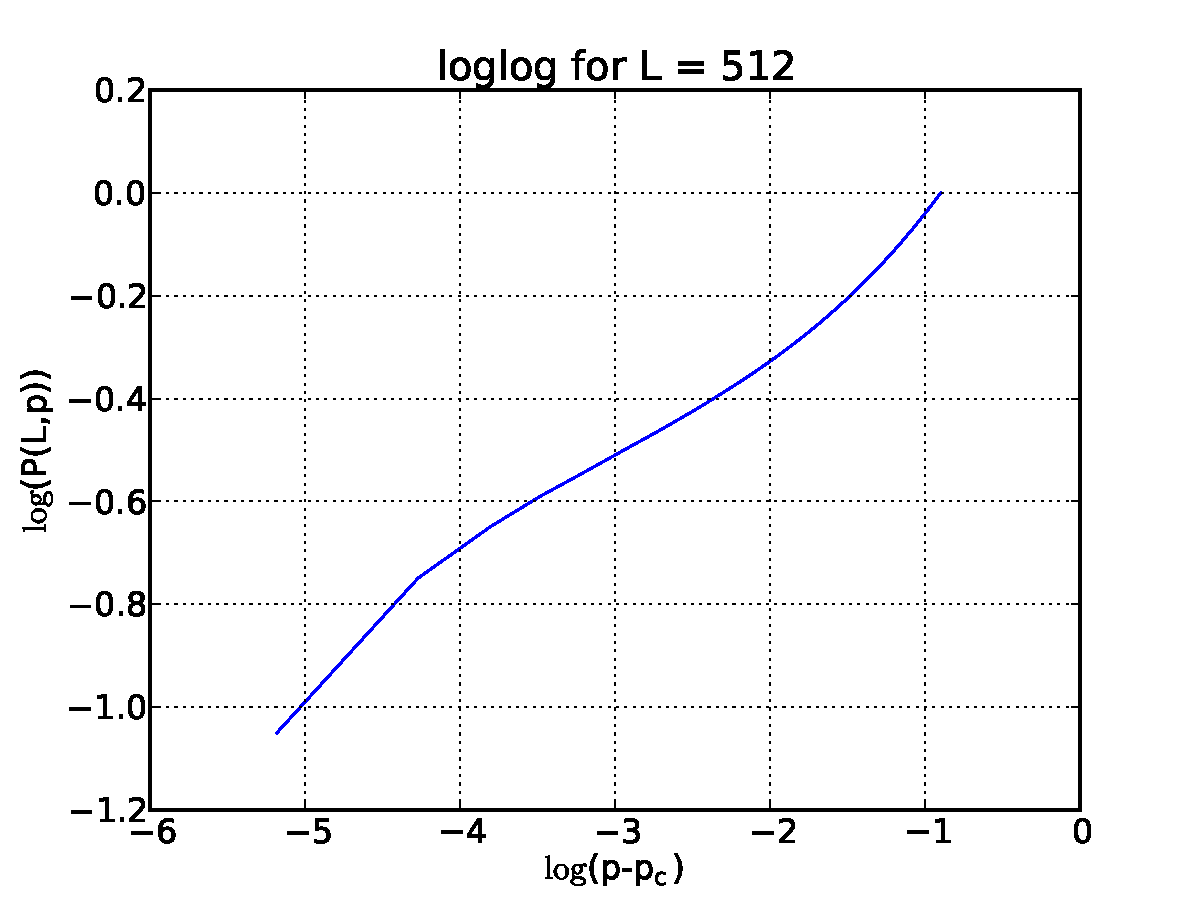
\includegraphics[width=0.45\textwidth]{../percolation/results/1a/P-vs-p-L512-nsamples500-loglog.pdf}
  % matrix.png: 800x600 pixel, 100dpi, 20.32x15.24 cm, bb=0 0 576 432
  \caption{loglog plot of the probability for a site to be part of the spanning cluster $\log P(p,L)$ plotted as a function of $\log (p-p_{c})$. This was found by sampling $P$ for $500$ random binary matrices for different values of $p$.}
  \label{fig:logP-vs-logp}
\end{figure}
By taking the derivative of this function (numerically) we get the plot shown in figure \ref{fig:logP-vs-logp-derivative}. From this plot we may read off the lowest value of the derivative as an estimate for $\beta$. In this case it appears to be about $\beta = 0.17$.
This is a bit higher than what is the expected value of $\beta = 0.14$.
\begin{figure}
  \centering
  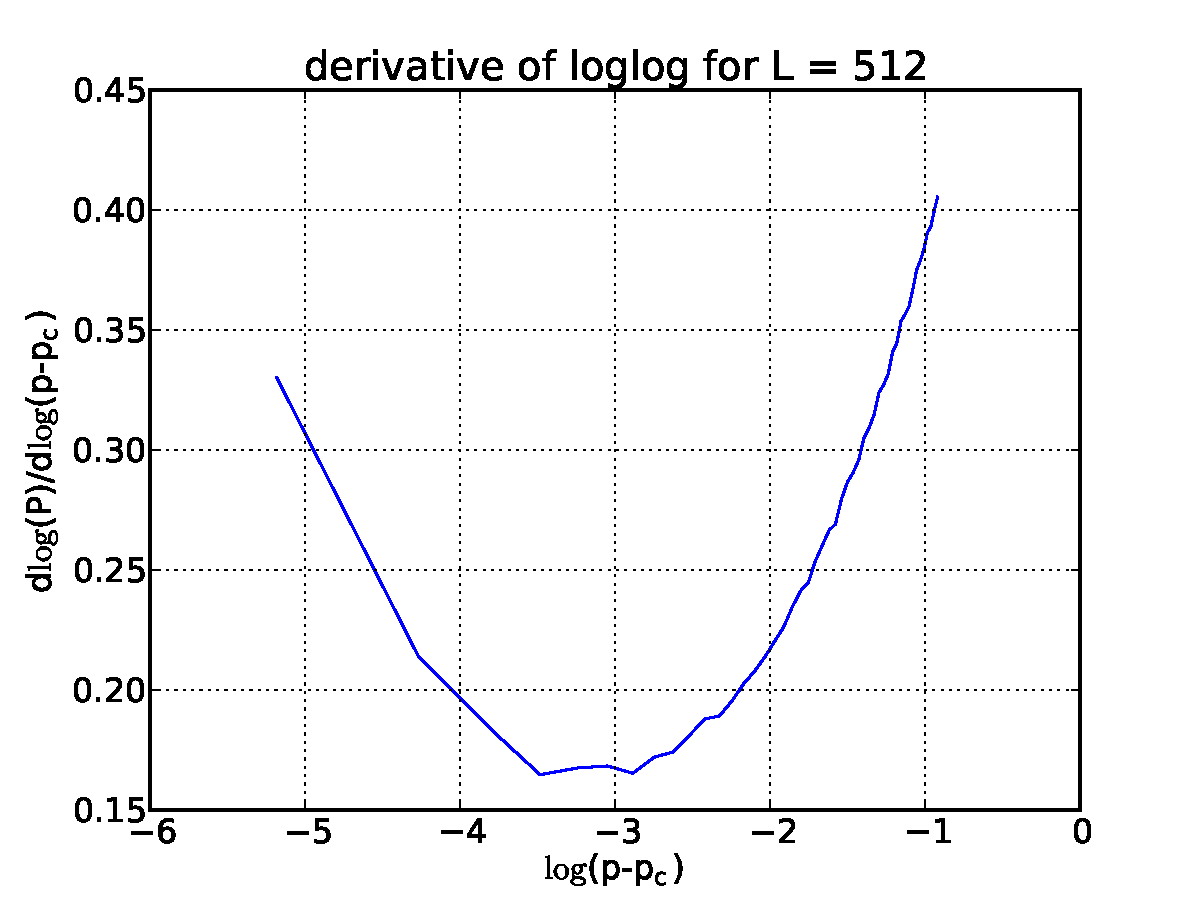
\includegraphics[width=0.45\textwidth]{../percolation/results/1a/P-vs-p-L512-nsamples500-loglogderivative.pdf}
  % matrix.png: 800x600 pixel, 100dpi, 20.32x15.24 cm, bb=0 0 576 432
  \caption{Derivative of the loglog plot of the probability for a site to be part of the spanning cluster $\log P(p,L)$ plotted as a function of $\log (p-p_{c})$. This was found by sampling $P$ for $500$ random binary matrices for different values of $p$.}
  \label{fig:logP-vs-logp-derivative}
\end{figure}

\subsection{Power-law distributions}

Before addressing cluster number densities, we need some tools to help us determine the exponent of power-law distributions. To do this, we are creating a set of random data points in Python:
\begin{lstlisting}
z = rand(1e6)**(-3+1)
\end{lstlisting}
This distribution is not suited for a regular histogram, but one with logarithmic binning will do. We may therefore construct a series of bin edges determined by Python's \textbf{logscale} function:
\begin{lstlisting}
mybins = histogram(z, bins=logspace(0,log10(z.max()),100))
\end{lstlisting}
We may now calculate the cumulative distribution function with data points within this binning by using Python's \textbf{cumsum} function and divide by the sum of all bins to find $P(Z > z)$:
\begin{lstlisting}
cumulativeDistribution = cumsum(mybins[0]) / float(sum(mybins[0]))
\end{lstlisting}
The result is shown in figure \ref{fig:powerlaw-cumulative-distribution}. Taking the derivative of the cumulative distribution gives us the actual distribution
\begin{equation}
  f_{Z}(z) = \frac{dP(Z > z)}{dz}
\end{equation} 
After calculating this, we take the logarithm of both $f_{Z}(z)$ and $z$ and calculate the incline of the curve. To find this exactly, we may take the numeric derivative and plot it as shown in figure \ref{fig:powerlaw-distribution-derivative}. Here we clearly see that the value for $\alpha$ is approximately $\alpha = -0.5$.
\begin{figure}
  \centering
  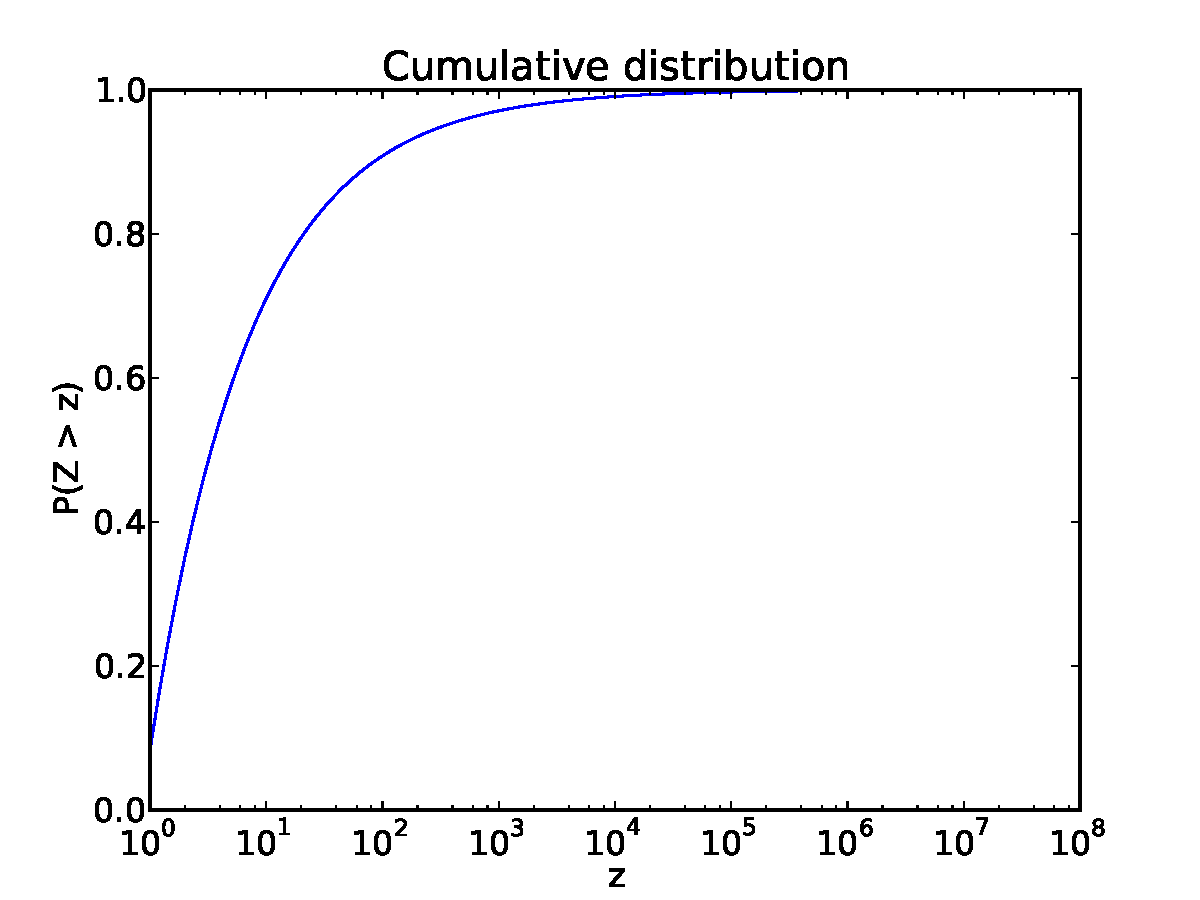
\includegraphics[width=0.45\textwidth]{../percolation/results/1c/cumulative-distribution.pdf}
  % matrix.png: 800x600 pixel, 100dpi, 20.32x15.24 cm, bb=0 0 576 432
  \caption{Cumulative distribution of the randomly selected data points.}
  \label{fig:powerlaw-cumulative-distribution}
\end{figure}
% \begin{figure}
%   \centering
%   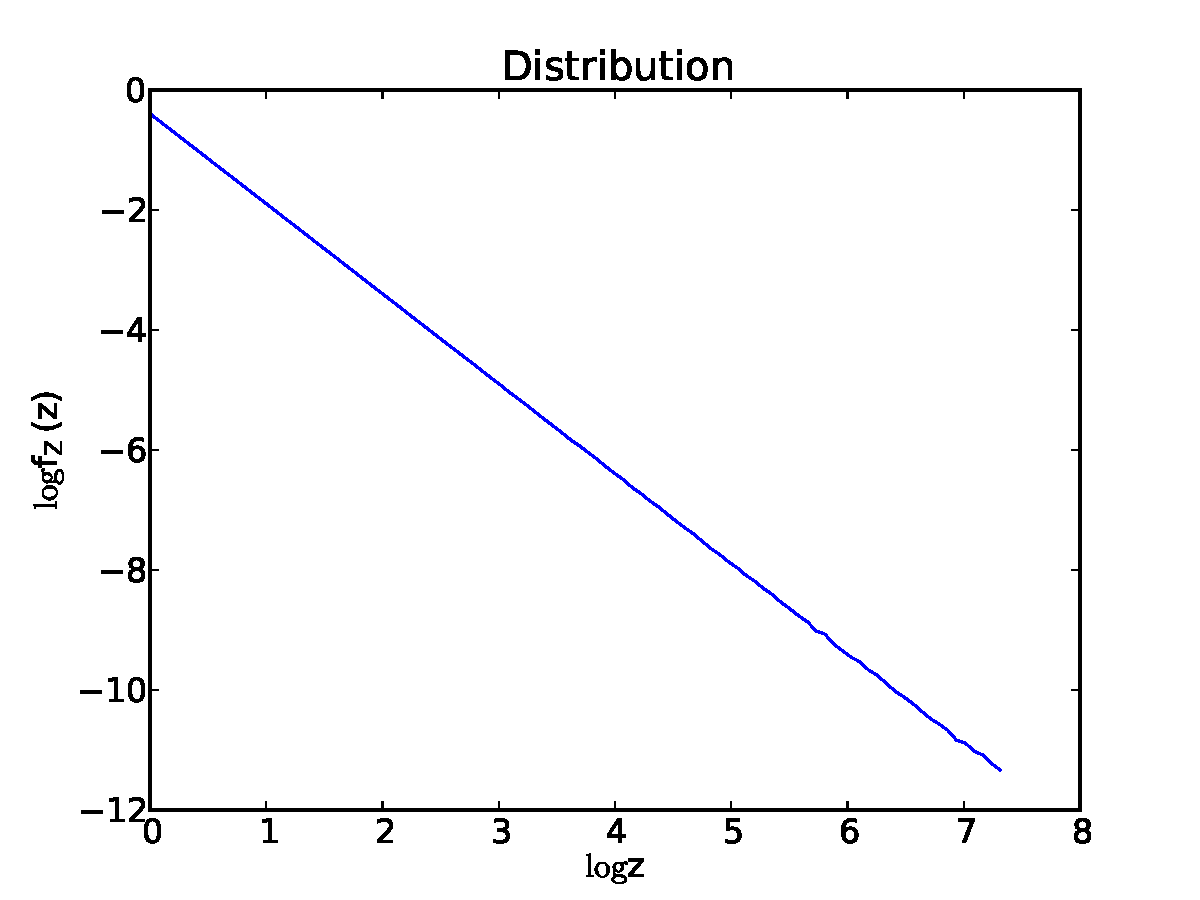
\includegraphics[width=0.45\textwidth]{../percolation/results/1c/distribution.pdf}
%   % matrix.png: 800x600 pixel, 100dpi, 20.32x15.24 cm, bb=0 0 576 432
%   \caption{Cumulative distribution of the randomly selected data points.}
%   \label{fig:powerlaw-distribution}
% \end{figure}
\begin{figure}
  \centering
  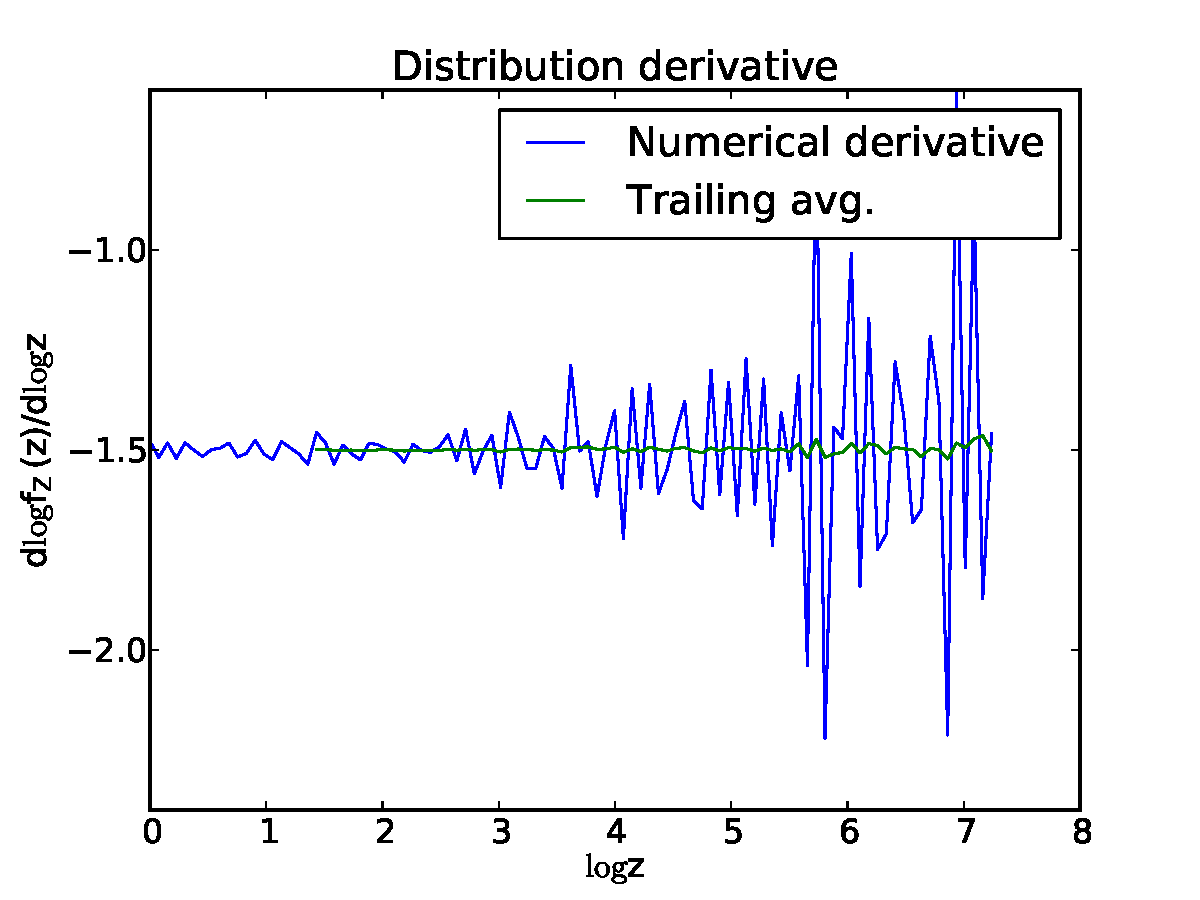
\includegraphics[width=0.45\textwidth]{../percolation/results/1c/distribution-derivative.pdf}
  % matrix.png: 800x600 pixel, 100dpi, 20.32x15.24 cm, bb=0 0 576 432
  \caption{Derivative of the logarithm of the cumulative distribution of the randomly selected data points.}
  \label{fig:powerlaw-distribution-derivative}
\end{figure}

With these tools in place, we can move on to calculating the cluster number density.

\subsection{Cluster number density}

The cluster number density $n(s,p)$ can be calculated by running the program we used in the first exercises to find the area for each cluster. Thereafter, we may find the number of occurences each area and weight each occurence by the area itself using the NumPy histogram function:
\begin{lstlisting}
currentBins = histogram(area, bins=bins, weights=area)[0]
\end{lstlisting}
Before doing this, we set the area of the spanning cluster to zero, just to make sure it does not contribute to the statistics.

If we now divide by the total area of the system, we will find the cluster number density for this specific system.

It is interesting to see what happens to the cluster number density as $p$ approaches $p_c$ from above and below. This is shown in figure \ref{fig:cluster-number-density}.

\begin{figure*}
  \centering
  \begin{subfigure}
  \centering
  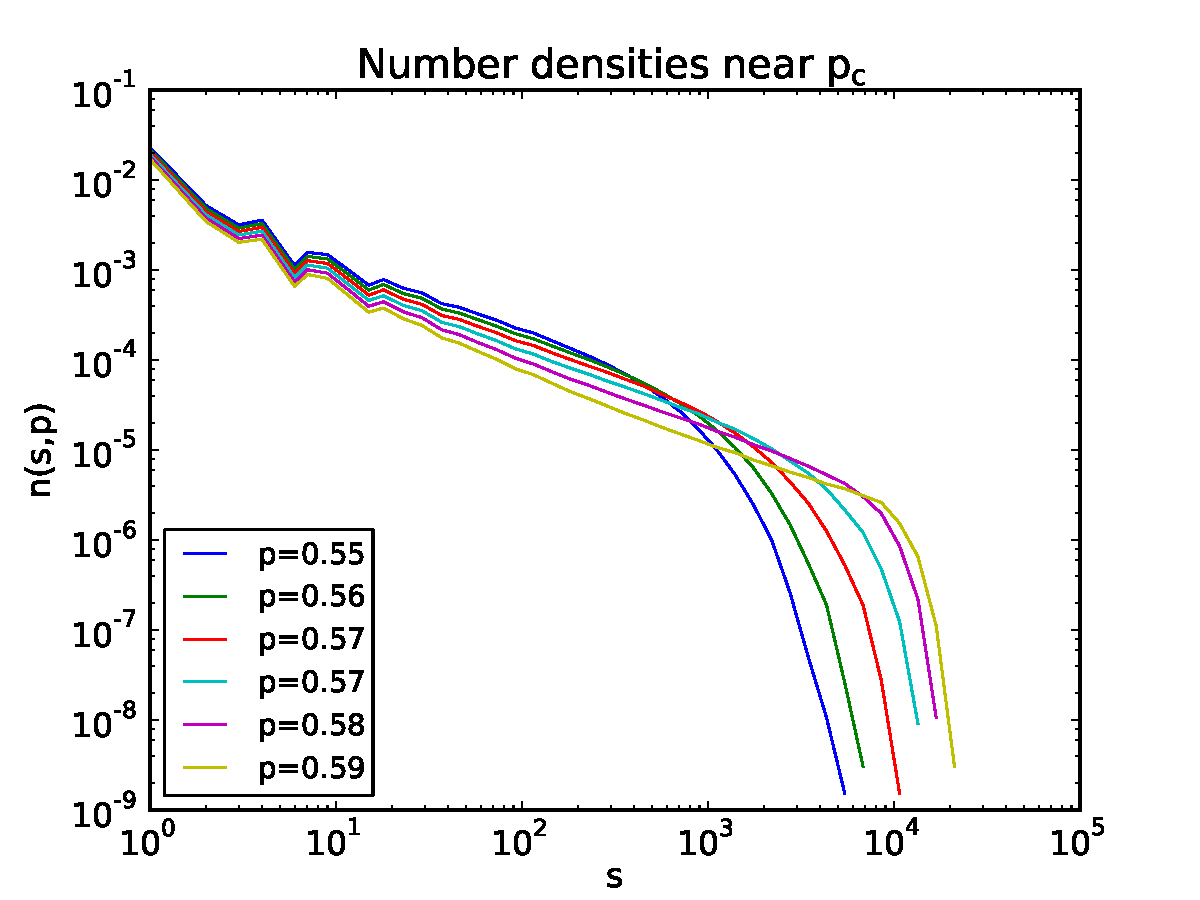
\includegraphics[width=0.45\textwidth]{../percolation/results/1e/n-vs-s-L256-nsamples10000-frombelow.pdf}
  \end{subfigure}
  \begin{subfigure}
  \centering
  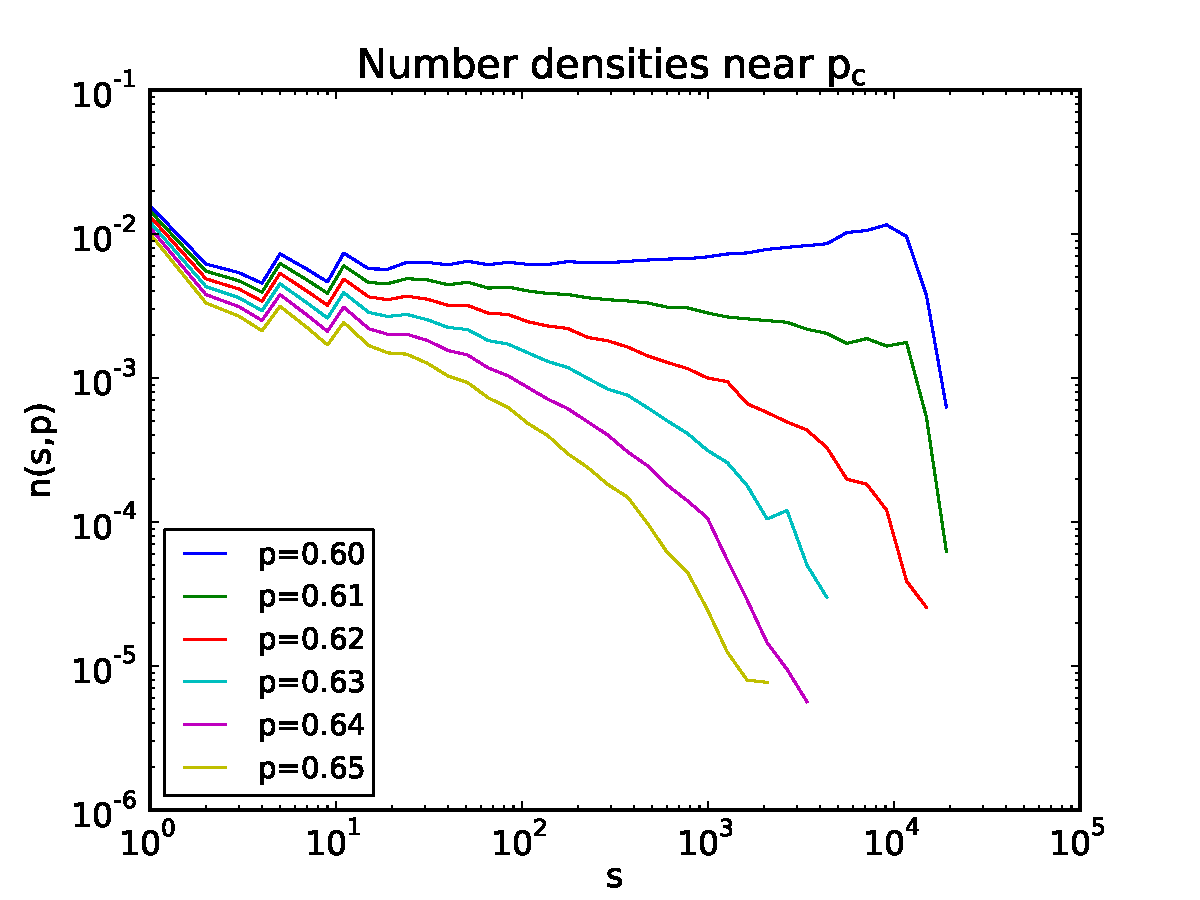
\includegraphics[width=0.45\textwidth]{../percolation/results/1e/n-vs-s-L256-nsamples10000-fromabove.pdf}
  \end{subfigure}
  \caption{loglog plot of the cluster number density for a system with $L=256$ using $1000$ samples for each value of $p$ as we approach $p_c$ from below (left) and above (right).}
  \label{fig:cluster-number-density}
\end{figure*}

\subsection{Finding $\tau$}

Furthermore, we are interested in seeing how the cluster number density at $p_c$ varies as a function of $s$ with the system size $L$. This is shown in figure \ref{fig:cluster-number-density-systemsize}.
%
\begin{figure}
  \centering
  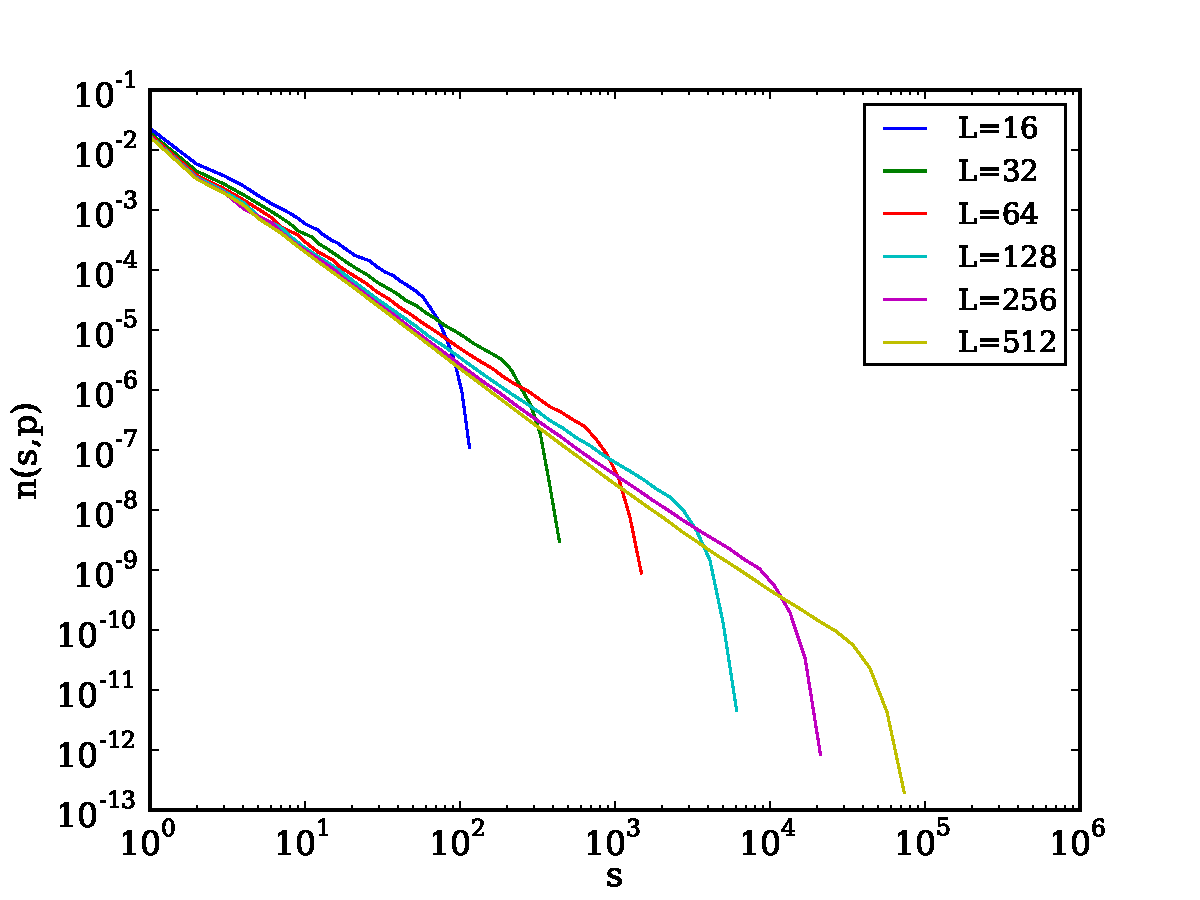
\includegraphics[width=0.45\textwidth]{../percolation/results/1f/n-vs-s-nsamples10000.pdf}
  % matrix.png: 800x600 pixel, 100dpi, 20.32x15.24 cm, bb=0 0 576 432
  \caption{Cluster number density $n(s,p_c)$ as function of $s$ for different system sizes.}
  \label{fig:cluster-number-density-systemsize}
\end{figure}
%
This is interesting because we assume that $F(s/s_{\xi}) = 1$ at $p_c$. This is what we find in 1-dimensional percolation theory, where $F(s/s_{\xi}) = e^{-s/s_{\xi}}$ and $s_{\xi} = -1 / \ln p$. When $p=p_{c}$, we get $s_{\xi} = \infty$ and assume something similar to happen in 2-dimensional systems. 

With $s/s_{\xi} = 0$, we get $F(s/s_{\xi}) = 1$ and the cluster number density at $p_{c}$ becomes only
\begin{equation}
  n(s,p_{c}) = s^{-\tau}
\end{equation} 
In all, we may use this to find $\tau$. In figure \ref{fig:cluster-number-density-systemsize} we see that with increasing $L$, there is a loglog trend towards a line with decreasing incline. If we could increase $L$ to extreme sizes, we may estimate the true value of $\tau$, but we are pretty much stuck with $L \leq 2048$ for this project. However, we could plot the estimate $\tau$ as a function of $L$ and see if this converges to the real value. 

This is done in figure \ref{fig:tau-vs-systemsize}.
%
\begin{figure}
  \centering
  \includegraphics[width=0.45\textwidth]{../percolation/results/1f/inclines-nsamples1000.pdf}
  % matrix.png: 800x600 pixel, 100dpi, 20.32x15.24 cm, bb=0 0 576 432
  \caption{$\tau$ fetched as incline from the different plots in figure \ref{fig:cluster-number-density-systemsize} as a function of system size $L$.}
  \label{fig:tau-vs-systemsize}
\end{figure}
%
We see that $\tau$ goes toward the true value of $\tau = 187/91 \approx 2.055$, but it would be hard to deduce this without knowing $\tau$ beforehand. In principle it is possible to use numerical methods to fit the curve in this figure, but it appeared somewhat tedious to do and was therefore not done in this project. The most clever method appears to be to use SciPy's \lstinlinebox{curve_fit} function. For now, the best we can guarantee from our data is that
\begin{equation}
  \tau > 1.94.
\end{equation} 

\subsection{Scaling of characteristic cluster size}

If we assume that the characteristic cluster size is proportional to $p - p_{c}$ through
\begin{equation}
  s_{\xi} \sim |p - p_{c}|^{1/\sigma}
\end{equation} 
we may plot $s_{\xi}$ against $|p-p_{c}$ to find $\sigma$. To do this, we first have to gather some data on the relation between the two.

We start out with the definition
\begin{equation}
  n(s,p) = s^{-\tau} F(s/s_{\xi})
\end{equation} 
to find
\begin{equation}
  \frac{n(s,p)}{n(s,p_{c})} = \frac{s^{-\tau}}{s^{-\tau}} \frac{F(s/s_{\xi})}{F(0)},
\end{equation} 
where we have used that $s_{\xi} = \infty$ at $p=p_{c}$. Further we assume that $F(0) = 1$ in 2 dimensions as it does in 1 dimension. This allows us to rewrite the ratio as
\begin{equation}
  \frac{n(s,p)}{n(s,p_{c})} = F(s/s_{\xi}).
\end{equation}
This is plotted in figure \ref{fig:scaling-ratio} as a function of $s$.

We don't yet know the function $F$, but we may use that we expect the function to go drastically towards $0$ as $s\to s_{\xi}$. If we intersect $F$ at a given value that will be close to where it goes to zero could therefore be a good estimate of $s_{\xi}$. If we do this for multiple systems with different $p$, we may finally plot $s_{\xi}$ as a function of $|p-p_{c}|$. This is shown in figure \ref{fig:sxi-vs-p} where $L = 1024$ has been used.
\begin{figure}
  \centering
  \includegraphics[width=0.45\textwidth]{../percolation/results/1g/n-vs-s-L1024-nsamples100-frombelow.pdf}
  % matrix.png: 800x600 pixel, 100dpi, 20.32x15.24 cm, bb=0 0 576 432
  \caption{$n(s,p)/n(s,p_{c})$ ratio as a function of $s$ for different $p$ for $L=1024$.}
  \label{fig:scaling-ratio}
\end{figure}
\begin{figure}
  \centering
  \includegraphics[width=0.45\textwidth]{../percolation/results/1g/sxi-L1024-nsamples100-frombelow.pdf}
  % matrix.png: 800x600 pixel, 100dpi, 20.32x15.24 cm, bb=0 0 576 432
  \caption{$s_{\xi}$ as a function of $p$ for $L=1024$.}
  \label{fig:sxi-vs-p}
\end{figure}

Taking the loglog of this plot and finding the incline lets us estimate $\sigma$ as $-1/\sigma$ of the incline. This was found to be
\begin{equation}
  \sigma = 0.394
\end{equation} 
which is pretty close to the true value of $\sigma = 0.396$. However, choosing a different set of $p$ might yield other results (as found by fellow students) as well as a different choice in system size.

\subsection{Mass scaling}

The mass $M(L)$ of the percolating cluster is shown in figure \ref{fig:mass-scaling}. This is once more an exponential function. Taking the logarithms of $M$ and $L$ and finding the incline gives us the scaling parameter $D$:
\begin{equation}
  M(L) = L^{D}
\end{equation}
It was found by taking the derivative of the loglog version of figure \ref{fig:mass-scaling} to be
\begin{equation}
  D \approx 1.86.
\end{equation} 
\begin{figure}
  \centering
  \includegraphics[width=0.45\textwidth]{../percolation/results/1h/M-vs-L-nsamples10000.pdf}
  % matrix.png: 800x600 pixel, 100dpi, 20.32x15.24 cm, bb=0 0 576 432
  \caption{Mass of the percolating cluster as a function of $L$.}
  \label{fig:mass-scaling}
\end{figure}

\subsection{Finite size scaling}



\end{document}
